\chapter{p 区（一）：硼族、碳族和氮族}\label{ch:b1:p-block-13-15}

我们呼吸的空气五分之四是氮气，植物却因缺氮而挨饿：
\ce{N#N} 三键极其牢固，几乎无物能将其打断。长期以来，
农作物的氮素主要来自粪肥、生长在豆科植物根部的细菌，
以及开采出的硝酸盐。二十世纪初，
氮气与氢气在铁催化剂上发生的反应
改变了这一局面：如今全球每年以氨的形式制得约 1.6 亿吨氮，
而人体内约一半的氮
都曾经过合成氨工厂。13、14 和 15 族元素是这段故事的主角：
氮和磷用于制造化肥，碳和
硅关乎生命与岩石，硼和铝用于玻璃与轻
质合金。本章借助前几章的工具逐一讨论它们。

\begin{recall}
碳的同素异形体，以及硅与二氧化硅的结构
（见\cref{ch:b1:crystals-ionic-covalent}）；氧化物的酸碱性
（见\cref{def:b1:s-block:oxide-character}）；氧化数与标准
电极电势（见\cref{ch:b1:nernst}）；两性氢氧化物
（见\cref{ch:b1:precipitation}）；由吉布斯自由能求平衡常数
（见\cref{ch:b1:extent-q-and-k}）。
\end{recall}
% ledger: usgs:N-world-2025

\begin{omfigure}
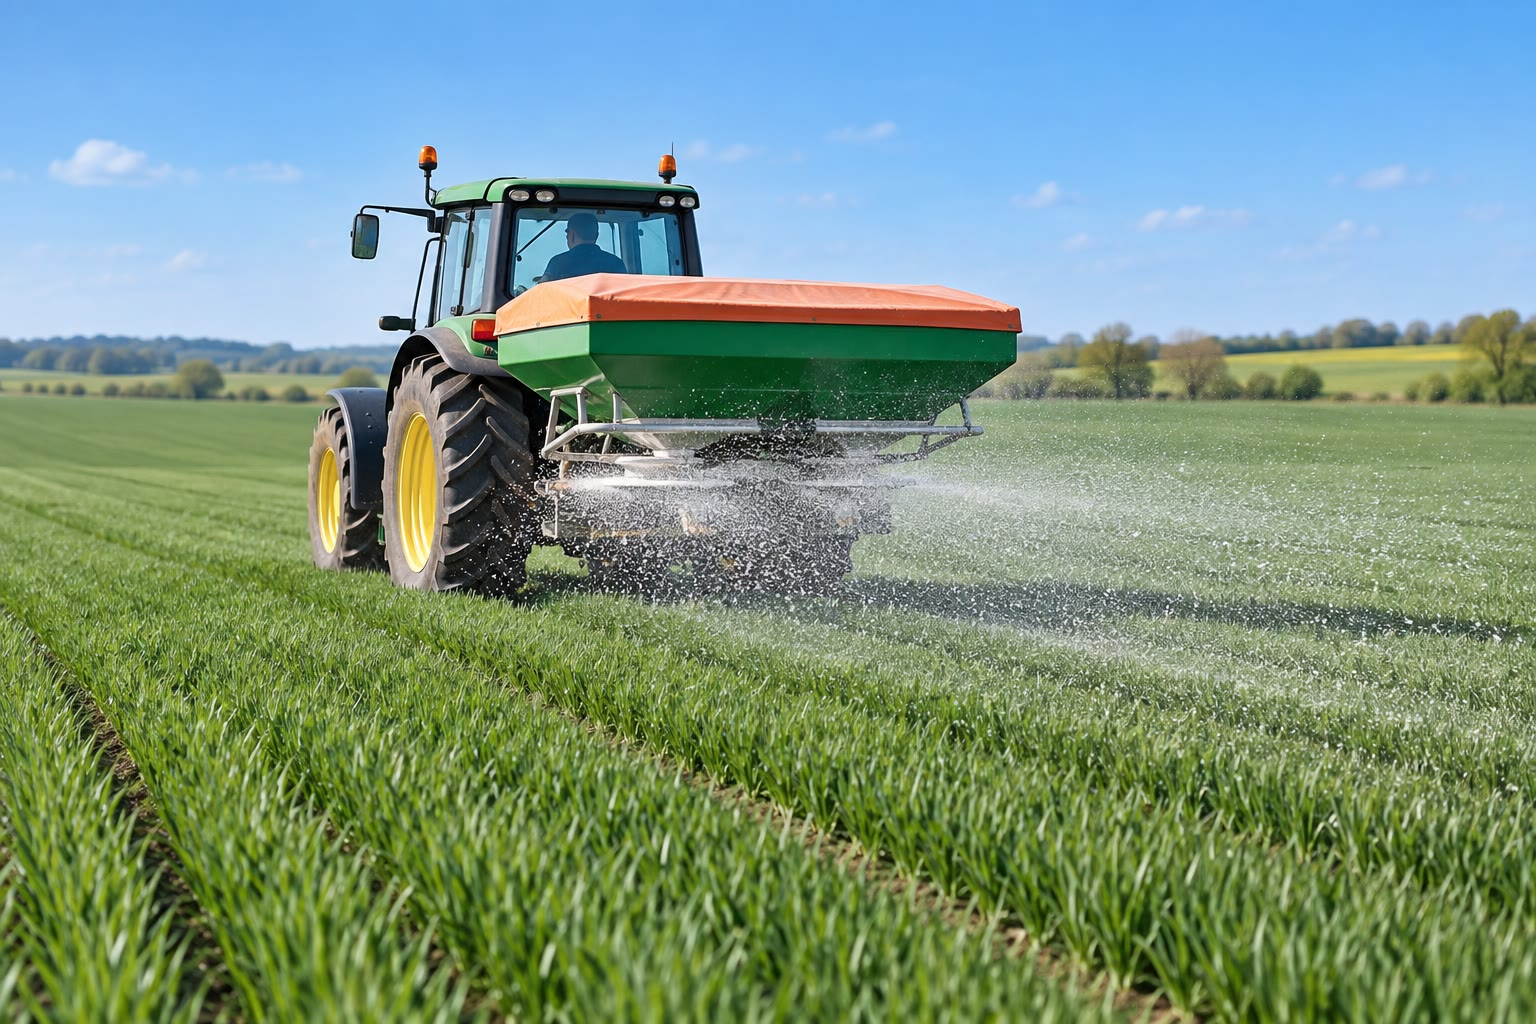
\includegraphics[width=0.55\linewidth]{images/book2/ai/b1-27-fertiliser-field.jpg}

{\small 在小麦田中撒施氮肥。其中大部分
由空气中的氮经哈伯–博施法制成。}
\end{omfigure}

\section{13 族：硼和铝}

硼是一种类金属，能形成八隅体不完整的共价化合物，
在 \ce{BF3} 和硼酸 \ce{B(OH)3} 中，硼有六个价电子，
并作为路易斯酸起作用（见\cref{ch:b1:lewis-resonance-vsepr}）。
硼酸是弱酸，但它并非靠失去质子，而是靠接受一个
氢氧根离子，即 \ce{B(OH)3 + 2H2O <=> B(OH)4- + H3O+}。硼砂是一种硼酸钠，
用于制造玻璃和洗涤剂。

\begin{definition}[含氧酸]\label{def:b1:p-block-13-15:oxoacid}
称\emph{含氧酸}\index{含氧酸}为这样一类酸，其酸性氢
原子与氧原子相连，而这些氧原子又与中心原子相连：
\ce{B(OH)3}, \ce{H2CO3}, \ce{HNO3} (\ce{HO-NO2}), \ce{H3PO4}
（\ce{(HO)3PO}）、\ce{H2SO4}。中心原子周围不与氢相连的氧原子越多，
酸性越强。
\end{definition}

铝位于硼的正下方，是一种金属，但其离子体积小、电荷高，
因而具有两性氧化物和两性氢氧化物（见\cref{sec:b1:precipitation:amphoteric}）。
其矿石为铝土矿，是氢氧化铝与氧化铁、
二氧化硅的混合物；2025 年全球开采铝土矿约 4.4 亿吨，
并从中精炼出约 1.5 亿吨氧化铝。
% ledger: usgs:bauxite-world-2025, usgs:alumina-world-2025

\begin{proposition}[拜耳法]\label{prop:b1:p-block-13-15:bayer}
热的浓氢氧化钠将铝土矿中的铝溶解为
\ce{Al(OH)4-}，并留下氧化铁（赤泥）；
过滤所得溶液经冷却并加入晶种，使纯净的 \ce{Al(OH)3} 沉淀，煅烧后得氧化铝，即
\ce{2Al(OH)3 -> Al2O3 + 3H2O}.
\end{proposition}

\begin{proof}
\ce{Al(OH)3(s) + OH- <=> Al(OH)4-} 在 \qty{25}{\celsius} 时的平衡常数为 $K = 10^{-1.23}$
（见\cref{ch:b1:precipitation}）：当 \ce{[OH-]} 较高时，
铝留在溶液中，而不具两性的氢氧化铁(III)
仍为固体（见\cref{exo:b1:precipitation:12}）。稀释与降温会降低
\ce{[OH-]}，并使反应商改变，从而对逆反应有 $Q > K$：
即氢氧化铝析出。煅烧脱去水分。
\end{proof}

随后，氧化铝在熔融冰晶石中通过电解还原为铝，
这一工业过程在本科二年级分册中讨论。

\begin{omfigure}
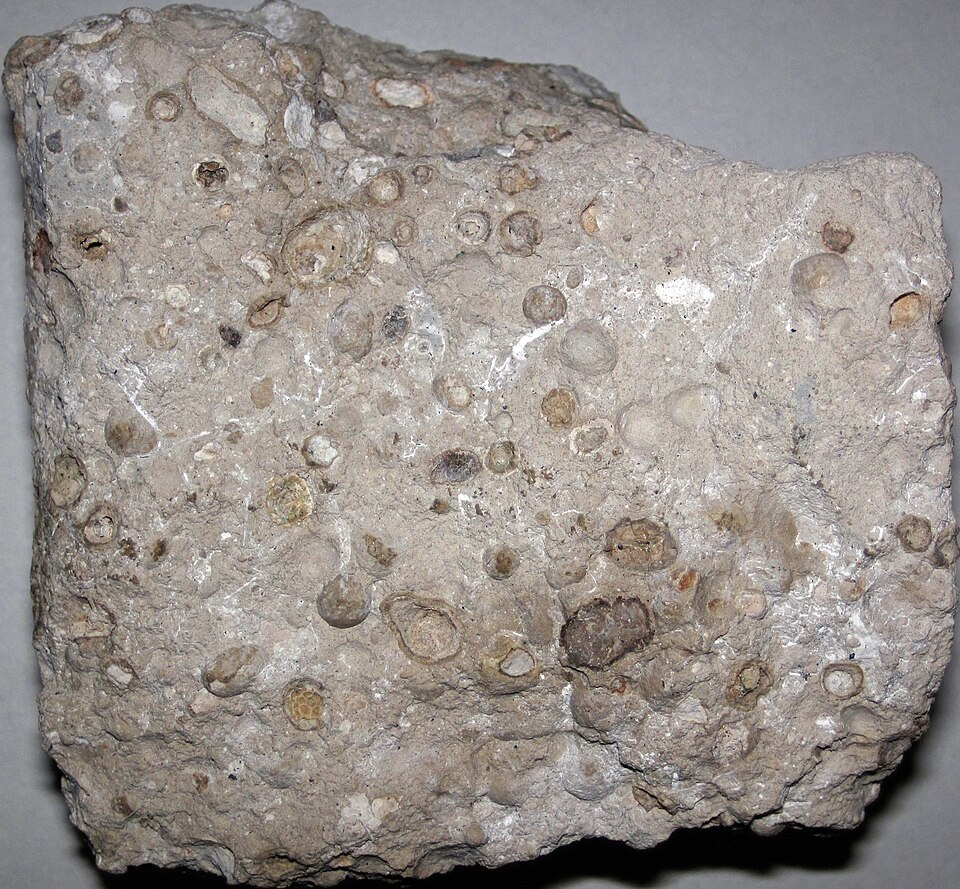
\includegraphics[height=3.6cm]{images/book2/bauxite.jpg}\hspace{0.4em}%
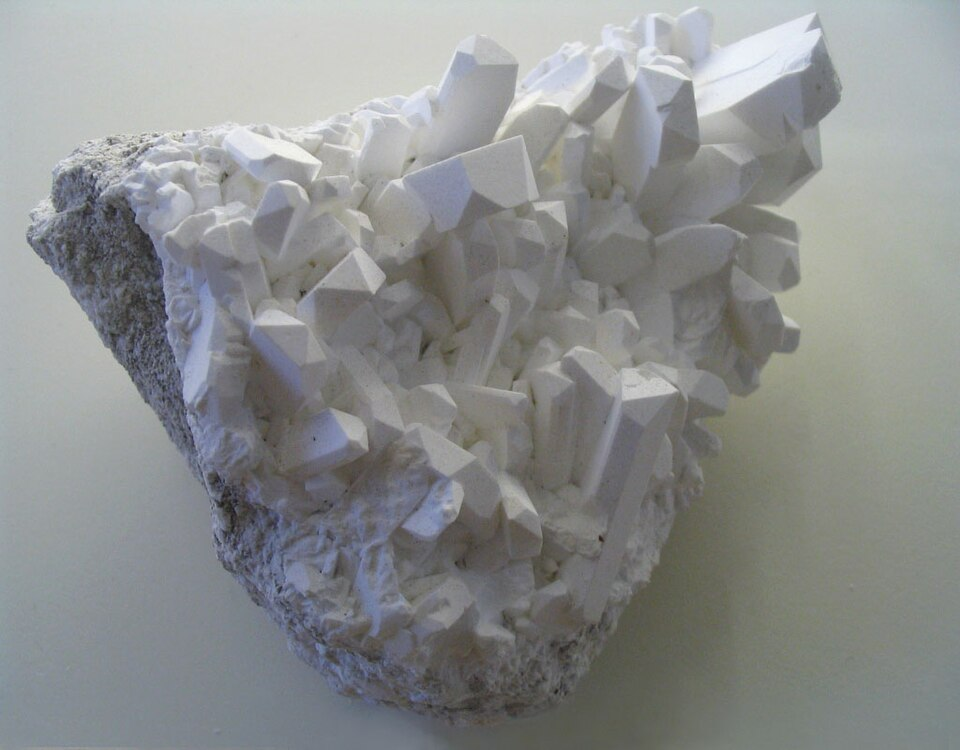
\includegraphics[height=3.6cm]{images/book2/borax.jpg}\hspace{0.4em}%
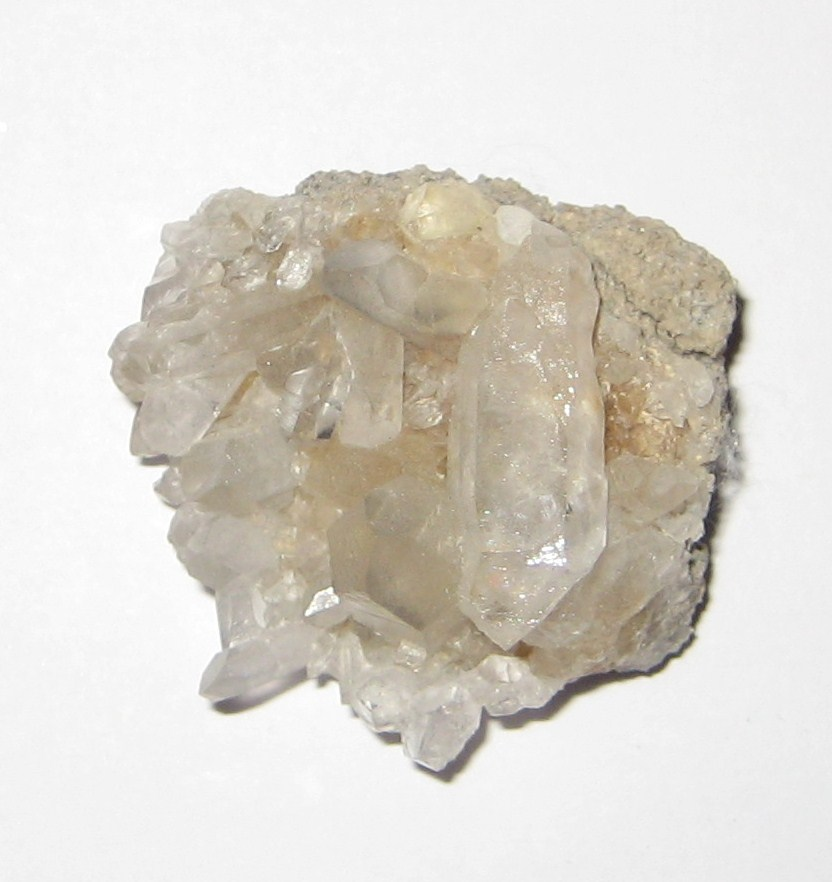
\includegraphics[height=3.6cm]{images/book2/quartz.jpg}\hspace{0.4em}%
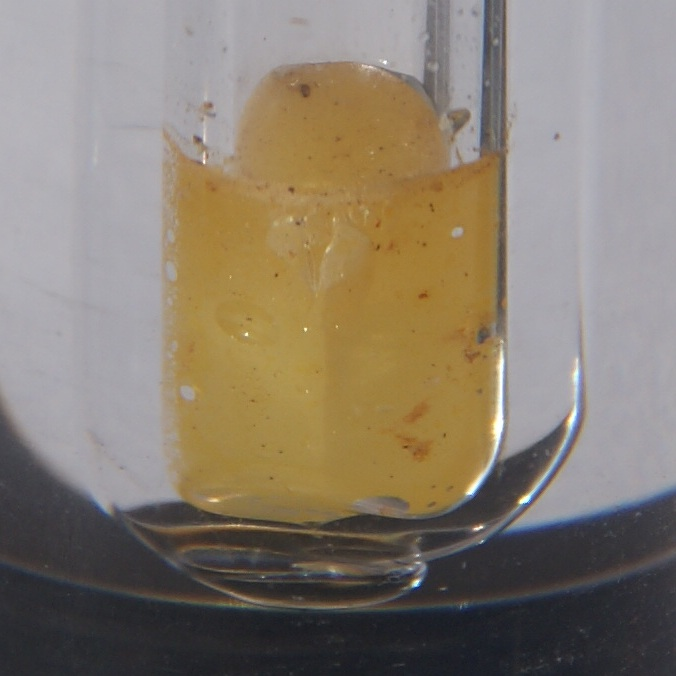
\includegraphics[height=3.6cm]{images/book2/white-phosphorus.jpg}

{\small 从左至右：豆状铝土矿（照片：James St. John，CC BY 2.0）；
硼砂晶体（照片：Aram Dulyan，公有领域）；一簇石英晶体，
\ce{SiO2}（照片：Stephanie Clifford，CC BY 2.0）；白磷，含少量
红磷，因遇空气会自燃而需保存于水中
（照片：Hi-Res Images of Chemical Elements，CC BY 3.0）。图片均来自维基共享资源。}
\end{omfigure}

\section{14 族：碳和硅}

碳和硅都能形成四个键，但方式不同。碳能形成
较强的双键：\ce{CO2} 是分子 \ce{O=C=O}，是一种气体。硅
几乎不形成双键：\ce{SiO2} 是由 \ce{SiO4} 四面体组成的共价网络，
各四面体共用全部顶点，构成坚硬的固体石英（见\cref{ch:b1:crystals-ionic-covalent}）。
二氧化碳是酸性氧化物，可生成碳酸、碳酸氢盐
和碳酸盐（见\cref{ch:b1:predominant-reaction}）；二氧化硅同样是酸性
氧化物，可被熔融碱侵蚀而生成硅酸盐。

\begin{proposition}[硅酸盐单元]\label{prop:b1:p-block-13-15:silicate-units}
硅酸盐由 \ce{SiO4} 四面体构成；四面体之间共用的顶点数
决定阴离子的化学式：无共用顶点时为 \ce{SiO4^4-}
（孤立四面体）；两个时为链状 $(\ce{SiO3})_n^{2n-}$；三个时为
层状 $(\ce{Si2O5})_n^{2n-}$；四个时为中性骨架 \ce{SiO2}。
\end{proposition}

\begin{proof}
共用氧原子各归两个四面体一半。共用
$k$ 个顶点的四面体完全拥有 $4 - k$ 个氧原子，另有 $k$ 个各按半计：$4 -
k/2$ 个氧原子，即每个硅原子所占的氧原子数。每个未共用的氧原子带电荷 $-1$（它
只有一个键），共用的氧原子则不带电；每个硅原子上的电荷为
$-(4 - k)$。$k = 0$：\ce{SiO4^4-}；$k = 2$：按每个硅原子计为 \ce{SiO3^2-}；
$k = 3$：\ce{SiO_{2.5}^-}，即 \ce{Si2O5^2-}；$k = 4$：\ce{SiO2}。
\end{proof}

\begin{omfigure}
\begin{tikzpicture}[font=\small, line join=round]
  % one SiO4 tetrahedron in perspective
  \begin{scope}
    \coordinate (t) at (0,1.2); \coordinate (a) at (-1.0,-0.5);
    \coordinate (b) at (1.0,-0.5); \coordinate (c) at (0.25,0.05);
    \draw[thick, omDef] (t) -- (a) -- (b) -- cycle; \draw[thick, omDef] (t) -- (b);
    \draw[dashed, omDef] (a) -- (c) -- (b) (t) -- (c);
    \foreach \p in {t,a,b,c} \shade[ball color=red!60] (\p) circle (0.16);
    \shade[ball color=gray!40] (0.06,0.18) circle (0.11);
    \node at (0,-1.2) {\ce{SiO4^4-}：单个四面体};
  \end{scope}
  % a chain of tetrahedra seen from above
  \begin{scope}[xshift=3.6cm]
    \foreach \i in {0,1,2,3} {
      \draw[thick, omDef, fill=omDef!10] (\i*1.1,0) -- (\i*1.1+0.55,0.95) -- (\i*1.1+1.1,0) -- cycle;
      \shade[ball color=red!60] (\i*1.1+0.55,0.95) circle (0.12);
      \shade[ball color=red!60] (\i*1.1+0.55,0.32) circle (0.10);
    }
    \foreach \i in {0,1,2,3,4} \shade[ball color=red!60] (\i*1.1,0) circle (0.12);
    \node[align=center] at (2.2,-1.0) {链状 $(\ce{SiO3})_n^{2n-}$：每个四面体 \\ 共用两个顶点（从上方看）};
  \end{scope}
\end{tikzpicture}

{\small 硅酸盐单元：孤立的 \ce{SiO4} 四面体（硅为灰色，
氧为红色），以及一条链，其中每个四面体与相邻者共用两个氧
原子。层状（三个共用顶点）构成云母和
黏土；骨架（四个共用顶点）构成石英。}
\end{omfigure}

\begin{definition}[惰性电子对效应]\label{def:b1:p-block-13-15:inert-pair}
\emph{惰性电子对效应}\index{惰性电子对效应}是指沿第 13 至 15 族向下，
比该族最高氧化态低两个单位的氧化态稳定性递增：
例如铊（I）比铊（III）稳定，铅（II）比铅（IV）稳定，铋（III）比铋（V）稳定。
重元素的 \textit{ns}$^2$ 电子对束缚很紧，
较少参与成键。
\end{definition}

该效应解释了为什么二氧化铅是一种强氧化剂
（$E^\circ(\ce{PbO2}/\ce{Pb^2+}) = 1.46$~V，见\cref{ch:b1:nernst}），而
碳（IV）和硅（IV）则是它们各自元素的稳定氧化态。

\section{第 15 族：氮}

\begin{proposition}[氮的阶梯]\label{prop:b1:p-block-13-15:nitrogen-ladder}
氮取遍 $-3$ 到 $+5$ 之间的每个氧化数：\ce{NH3} 和
\ce{NH4+}（$-$III）、\ce{N2H4}（$-$II）、\ce{NH2OH}（$-$I）、\ce{N2}（0）、
\ce{N2O}（$+$I）、\ce{NO}（$+$II）、\ce{HNO2} 和 \ce{NO2-}（$+$III）、
\ce{NO2}（$+$IV）、\ce{HNO3} 和 \ce{NO3-}（$+$V）。
\end{proposition}

\begin{proof}
对每个化学式应用\cref{prop:b1:nernst:on-rules}中的规则，取 H 为
$+$I，O 为 $-$II：在 \ce{N2H4} 中 $2x + 4 = 0$；在 \ce{NO2-} 中 $x - 4 =
-1$；依此类推。
\end{proof}

\begin{definition}[固氮]\label{def:b1:p-block-13-15:nitrogen-fixation}
\emph{固氮}\index{固氮}是指任何能把空气中的
氮气转化为可供生物或工业利用的化合物（氨、硝酸盐）的过程：
细菌的生物固氮、
闪电固氮和氨的工业合成。
\end{definition}

哈伯–博施法使氮气与氢气在铁
催化剂上化合，即 \ce{N2 + 3H2 <=> 2NH3}。该反应在室温下热力学上有利
（\qty{25}{\celsius} 时 $K = 10^{5.8}$，由氨的生成吉布斯自由能算得），
但反应太慢；催化剂只有在高温下才起作用，而
兼顾速率与产率的温度与压强的选择，
在本科二年级分册中确定。氨随后
通过奥斯特瓦尔德法氧化为硝酸。
% ledger: dfg:NH3_g

\begin{omfigure}
\begin{tikzpicture}[font=\small, >={Stealth}, box/.style={draw, rounded corners, fill=omDef!8, align=center, minimum height=0.9cm}]
  \node[box] (air) at (0,0) {空气 \\\ce{N2}};
  \node[box] (gas) at (0,-1.6) {天然气 \\\ce{H2}};
  \node[box] (hb) at (3.4,-0.8) {哈伯–博施法 \\铁催化剂};
  \node[box] (ox1) at (7.3,-0.8) {铂铑网 \\\ce{NH3} $\to$ \ce{NO}};
  \node[box] (ox2) at (11.0,-0.8) {氧化 \\吸收 \\\ce{NO} $\to$ \ce{NO2} $\to$ \ce{HNO3}};
  \draw[->, thick] (air) -- (hb);
  \draw[->, thick] (gas) -- (hb);
  \draw[->, thick] (hb) -- node[above] {\ce{NH3}} (ox1);
  \draw[->, thick] (ox1) -- node[above] {\ce{NO}} (ox2);
  \draw[->, thick] (ox2.south) -- ++(0,-0.6) node[below] {\ce{HNO3}};
  \draw[->, thick] (hb.south) -- ++(0,-0.9) node[below] {\ce{NH3}（化肥）};
  \draw[->, thick] (ox2.north) -- ++(0,0.5) -| node[pos=0.25, above] {\ce{NO} 循环利用} (ox1.north);
\end{tikzpicture}

{\small 从空气到硝酸：合成氨，随后是奥斯特瓦尔德法的
三个步骤。}
\end{omfigure}

\begin{method}[配平串联工业反应方程式]\label{met:b1:p-block-13-15:ostwald-balance}
\begin{enumerate}
  \item 逐步配平：（1）\ce{4NH3 + 5O2 -> 4NO + 6H2O};
        （2）\ce{2NO + O2 -> 2NO2}；（3）\ce{3NO2 + H2O -> 2HNO3 + NO}。
  \item 将各步乘以适当系数，使生成的每种反应中间体都被消耗
        （第 3 步生成的 \ce{NO} 返回第 2 步）。
  \item 相加：若 NO 完全循环利用，总方程式为
        \ce{NH3 + 2O2 -> HNO3 + H2O}，即每个氨对应一分子硝酸。
  \item 质量衡算用总方程式，
        各反应器的设计用各步反应。
\end{enumerate}
\end{method}

\begin{history}[弗里茨·哈伯]
\begin{minipage}[t]{0.18\linewidth}\vspace{0pt}
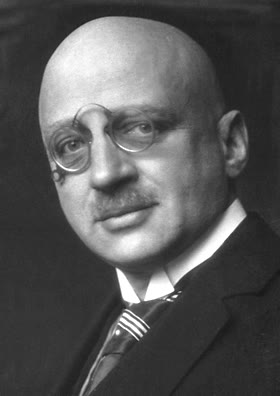
\includegraphics[width=\linewidth]{images/book2/haber.jpg}
\end{minipage}\hfill
\begin{minipage}[t]{0.78\linewidth}\vspace{0pt}
弗里茨·哈伯证明，氨可在压强下借助催化剂由氮气与氢气合成；
卡尔·博施则将实验室反应变为工业过程。
哈伯获得 1918 年诺贝尔化学奖。
同一个人还主持了氯气作为武器的首次大规模使用，
发生在第一次世界大战中：养活半个人类的化学，
与致人死亡的化学之间，只隔着化学家的选择。
（照片：The Nobel Foundation，1919 年发表，公有领域，
维基共享资源。）
\end{minipage}
\end{history}

\section{磷与同族元素的递变}

位于氮之下的磷不形成 \ce{P#P} 三键：白磷
由 \ce{P4} 四面体构成，张力大、活性高（它
在空气中会自燃，需保存于水中）；红磷
为聚合物，活性低得多。燃烧磷得到 \ce{P4O10}，它是
常见氧化物中酸性最强的，与水反应生成磷酸，
$\mathrm{p}K_a$ 为 2.15、7.21、12.34（见\cref{ch:b1:predominant-reaction}）。
2025 年开采的磷矿约 2.5 亿吨，经
硫酸处理后制成磷肥。
% ledger: usgs:phosphate-world-2025

沿族向下，元素金属性增强（硼至铊、
碳至铅、氮至铋），其氧化物碱性增强，
低氧化数更稳定，即惰性电子对效应。
沿周期向右，氧化物酸性增强，由碱性的 \ce{Na2O}
变为磷、硫的酸性氧化物。

\section{练习}

\begin{exercise}[$\star$]\label{exo:b1:p-block-13-15:1}
求下列物质中氮的氧化数：\ce{NH4NO3}（两个氮原子分别计算）、
\ce{N2O5}、\ce{HNO2}、\ce{N2H4} 和 \ce{Mg3N2}。
\end{exercise}

\begin{exercise}[$\star$]\label{exo:b1:p-block-13-15:2}
画出 \ce{BF3}、\ce{NH3} 及加合物
\ce{F3B-NH3} 的路易斯结构，并判断路易斯酸和路易斯碱。
\end{exercise}

\begin{exercise}[$\star$]\label{exo:b1:p-block-13-15:3}
写出 \ce{CO2}、\ce{SiO2}（熔融态）与 \ce{P4O10} 分别与
氢氧化钠的反应，以及 \ce{Al2O3} 分别与酸、碱的反应。
\end{exercise}

\begin{exercise}[$\star$]\label{exo:b1:p-block-13-15:4}
计算反应 \ce{N2 + 3H2 <=> 2NH3} 在
\qty{25}{\celsius} 下的平衡常数，已知 $\Delta_f G^\circ(\ce{NH3}) =
\qty{-16.45}{kJ/mol}$。
\end{exercise}

\begin{exercise}[$\star\star$]\label{exo:b1:p-block-13-15:5}
利用\cref{prop:b1:p-block-13-15:silicate-units}的计数方法，给出
由六个四面体构成、每个四面体共享两个顶点的环（如绿柱石中）的化学式，
以及双链的化学式，其中一半四面体共享两个顶点，
另一半共享三个顶点。
\end{exercise}

\begin{exercise}[$\star\star$]\label{exo:b1:p-block-13-15:6}
计算一吨铝土矿中所得氧化铝的质量，该铝土矿含
\ce{Al(OH)3} 质量分数为 \qty{55}{\percent}，
回收率为 \qty{92}{\percent}。
\end{exercise}

\begin{exercise}[$\star\star$]\label{exo:b1:p-block-13-15:7}
证明硼酸是路易斯酸而非布朗斯特酸，并
说明其溶液为何仍呈酸性。
\end{exercise}

\begin{exercise}[$\star\star$]\label{exo:b1:p-block-13-15:8}
利用氧化数配平氨被氧化为 \ce{NO} 的反应，
并给出每个 \ce{NH3} 转移的电子数。
\end{exercise}

\begin{exercise}[$\star\star$]\label{exo:b1:p-block-13-15:9}
硝酸铵由氨与硝酸制得。写出该反应，并
计算每吨硝酸铵所需氨的质量（包括制备硝酸所需的氨，
以及中和所需的氨）。
\end{exercise}

\begin{exercise}[$\star\star\star$]\label{exo:b1:p-block-13-15:10}
解释氮为何是双原子气体、磷为何是
由 \ce{P4} 分子组成的固体，以及二氧化碳为何是气体、二氧化硅为何是固体，
并利用第二周期与第三周期原子之间 $\pi$ 键的强度加以说明。
\end{exercise}

\begin{exercise}[$\star\star\star$]\label{exo:b1:p-block-13-15:11}
利用标准电极电势证明，在酸性条件下二氧化铅能将氯离子氧化为氯气，
而二氧化硅无此作用。
并将此结果与惰性电子对效应联系起来。
\end{exercise}

\begin{exercise}[$\star\star\star$]\label{exo:b1:p-block-13-15:12}
2025 年全世界以氨形式生产的氮约 1.6 亿吨。
这些氮相当于多少质量的氨？其中含有多少质量的氢？
这些氢主要来自何处？
\end{exercise}

\section{周末问题：从空气到化肥}

\begin{problem}[{周末问题——氮的三键、氨的合成、
硝酸生产的三个步骤、硝酸铵，
以及由一吨氨可得的硝酸质量}]
\label{pb:b1:p-block-13-15:1}
某化肥厂将氨转化为硝酸和
硝酸铵。摩尔质量（\unit{g/mol}）：\ce{N2} 28.0、\ce{H2} 2.0、\ce{NH3}
17.0、\ce{HNO3} 63.0、\ce{NH4NO3} 80.0、\ce{O2} 32.0；
已知 $\Delta_f G^\circ(\ce{NH3(g)}) = \qty{-16.45}{kJ/mol}$，
温度为 \qty{25}{\celsius}。

\medskip
\noindent\textbf{第一部分——氮。}
\begin{enumerate}
  \item 画出 \ce{N2} 的路易斯结构，并说明其为何化学性质不活泼。
  \item 求 \ce{N2}、\ce{NH3}、\ce{NO}、
        \ce{NO2}、\ce{HNO3} 和 \ce{NH4NO3} 中 N 的氧化数。
  \item 列举三种自然或工业固氮的方式。
  \item 为什么植物不能直接利用 \ce{N2}？
  \item 在合成氨中，哪种元素被氧化，
        哪种被还原？
  \item 写出合成氨的反应。
\end{enumerate}

\medskip
\noindent\textbf{第二部分——氨。}
\begin{enumerate}[resume]
  \item 计算合成反应在
        \qty{25}{\celsius} 时的平衡常数。
  \item 为什么合成仍要在高温、借助催化剂的条件下进行？
  \item 计算生产一吨氨所需的 \ce{N2} 和 \ce{H2}
        的质量。
  \item 空气（按体积计含 \qty{78}{\percent} 的 \ce{N2}，视为理想气体，
        在 \qty{25}{\celsius}、\qty{1}{bar} 下）体积为多少时含有这些氮气？
  \item 氢气从何而来？
  \item 为什么有些国家直接将氨用作化肥，
        而它又为何常先被转化？
\end{enumerate}

\medskip
\noindent\textbf{第三部分——硝酸。}
\begin{enumerate}[resume]
  \item 用氧化数配平第 1 步：\ce{NH3 + O2 -> NO + H2O}。 % ce-unbalanced-ok
  \item 配平第 2 步：\ce{NO + O2 -> NO2}。 % ce-unbalanced-ok
  \item 配平第 3 步：\ce{NO2 + H2O -> HNO3 + NO}。这属于哪一类 % ce-unbalanced-ok
        氧化还原反应？
  \item 将各步合并，并使 NO 完全循环利用，
        得到总反应方程式。
  \item 计算每吨氨消耗的氧气质量。
  \item 第 1 步为什么使用铂铑合金网？
\end{enumerate}

\medskip
\noindent\textbf{第四部分——硝酸铵与质量衡算。}
\begin{enumerate}[resume]
  \item 写出硝酸铵的生成反应。
  \item 需要将多少比例的氨转化为硝酸，
        才能只生成硝酸铵？
  \item 计算由一吨氨按此方式分配所得到的
        硝酸铵质量。
  \item 硝酸铵中含氮的质量分数是多少？
  \item 为什么硝酸铵必须远离燃料和热源储存？
  \item 计算由一吨氨可得到的硝酸质量，
        （完全转化）。
\end{enumerate}
\end{problem}
